\documentclass[12pt, titlepage]{article}

\usepackage{booktabs}
\usepackage{tabularx}
\usepackage{hyperref}
\usepackage{graphicx}
\usepackage{longtable}
\usepackage[utf8]{inputenc}
\usepackage[T1]{fontenc}
\usepackage{lmodern}
\usepackage{parskip}
\hypersetup{
    colorlinks,
    citecolor=black,
    filecolor=black,
    linkcolor=red,
    urlcolor=blue
}

\usepackage[round]{natbib}

%% Comments

\usepackage{color}

\newif\ifcomments\commentstrue %displays comments
%\newif\ifcomments\commentsfalse %so that comments do not display

\ifcomments
\newcommand{\authornote}[3]{\textcolor{#1}{[#3 ---#2]}}
\newcommand{\todo}[1]{\textcolor{red}{[TODO: #1]}}
\else
\newcommand{\authornote}[3]{}
\newcommand{\todo}[1]{}
\fi

\newcommand{\wss}[1]{\authornote{blue}{SS}{#1}} 
\newcommand{\plt}[1]{\authornote{magenta}{TPLT}{#1}} %For explanation of the template
\newcommand{\an}[1]{\authornote{cyan}{Author}{#1}}

%% Common Parts

\newcommand{\progname}{ProgName} % PUT YOUR PROGRAM NAME HERE
\newcommand{\authname}{Team \#, Team Name
\\ Student 1 name
\\ Student 2 name
\\ Student 3 name
\\ Student 4 name} % AUTHOR NAMES                  

\usepackage{hyperref}
    \hypersetup{colorlinks=true, linkcolor=blue, citecolor=blue, filecolor=blue,
                urlcolor=blue, unicode=false}
    \urlstyle{same}
                                


\begin{document}

\title{Verification and Validation Report: \progname} 
\author{\authname}
\date{\today}
	
\maketitle

\pagenumbering{roman}

\section{Revision History}

\begin{tabularx}{\textwidth}{p{3cm}p{2cm}X}
\toprule {\bf Date} & {\bf Version} & {\bf Notes}\\
\midrule
Date 1 & 1.0 & Notes\\
Date 2 & 1.1 & Notes\\
\bottomrule
\end{tabularx}

~\newpage

\section{Symbols, Abbreviations and Acronyms}

\renewcommand{\arraystretch}{1.2}
\begin{tabular}{l l} 
  \toprule		
  \textbf{symbol} & \textbf{description}\\
  \midrule 
  TPG & Tangled Program Graphs\\
  DNNs & Deep Neural Networks\\
  RL & Reinforcement Learning\\
  SRS & Software Requirement Specification\\
  FR & Functional Requirement\\
  NFR & Non-Functional Requirement\\
  SLN & System Level Number\\
  VnV & Verification and Validation\\
  \bottomrule
\end{tabular}\\

% \wss{symbols, abbreviations or acronyms -- you can reference the SRS tables if needed}

\newpage

\tableofcontents

\listoftables %if appropriate

\listoffigures %if appropriate

\newpage

\pagenumbering{arabic}

This document cohesively summarizes the results of each test as specified in the \href{https://github.com/TPGEngine/tpg/blob/main/docs/VnVPlan/VnVPlan.pdf}{VnV Plan} documentation.

\section{Functional Requirements Evaluation}

\subsection{MuJoCo Integration}

\begin{center}
\begin{longtable}{|p{2cm}|p{8cm}|p{2cm}|}
  \caption{MuJoCo Integration Tests} \\
\hline
\textbf{Test Id} & \textbf{Notes} & \textbf{Result} \\
\hline
\endfirsthead
\hline
\textbf{Test Id} & \textbf{Notes} & \textbf{Result} \\
\hline
\endhead
FR-SLN1 & When executing the appropriate script, all MuJoCo environments can be run. The best-performing agent within the policy can be visualized using OpenGL or an MP4 file. & Pass \\
\hline
FR-SLN2 & MuJoCo environments within the TPG framework can be successfully run within the Digital Research Alliance, enabling research to be conducted by executing experiments. & Pass \\
\hline
\end{longtable}
\end{center}

\subsection{Experiment Visualization}

\begin{center}
  \begin{longtable}{|p{2cm}|p{8cm}|p{2cm}|}
    \caption{Experiment Visualization Tests} \\
  \hline
  \textbf{Test Id} & \textbf{Notes} & \textbf{Result} \\
  \hline
  \endfirsthead
  \hline
  \textbf{Test Id} & \textbf{Notes} & \textbf{Result} \\
  \hline
  \endhead
  FR-SLN3 & When an experiment is running or finished training, the best performing policy can be visualized using the TPG CLI tool. & Pass \\
  \hline
  \end{longtable}
\end{center}

\section{Nonfunctional Requirements Evaluation}

\subsection{Usability}
		
\subsection{Performance}

\subsection{Operational and Environmental}

\begin{center}
  \begin{longtable}{|p{4cm}|p{4cm}|}
  \caption{Operational and Environmental Tests} \\
  \hline
  \textbf{Test Id} & \textbf{Result} \\
  \hline
  \endfirsthead
  \hline
  \textbf{Test Id} & \textbf{Result} \\
  \hline
  \endhead
  NFR-SLR6 & Pass \\
  \hline
  \end{longtable}
\end{center}

For NFR-SLN6, TPG now supports contributions from macOS, Windows, and Linux developers.
Previously, only Linux was supported because TPG used SCons for C++ builds and Linux-specific dependencies from \href{https://gitlab.cas.mcmaster.ca/kellys32/tpg/-/blob/main/requirements.txt}{requirements.txt}.
With VSCode Dev Containers, a Linux development environment is automatically launched for all developers, ensuring a standardized setup.
Simply follow the \href{https://gitlab.cas.mcmaster.ca/kellys32/tpg/-/wikis/home}{Wiki} instructions to download all necessary Linux dependencies and build the C++ code reliably. Onboarding on a Macbook has been reduced from 2 weeks to just 5 minutes.

\subsection{Compliance}

\begin{center}
\begin{longtable}{|p{4cm}|p{4cm}|}
\caption{Compliance Tests} \\
\hline
\textbf{Test Id} & \textbf{Result} \\
\hline
\endfirsthead
\hline
\textbf{Test Id} & \textbf{Result} \\
\hline
\endhead
NFR-SLR9 & Pass \\
\hline
\end{longtable}
\end{center}

The modified codebase is successfully analyzed using Clang-Tidy and Clang-Format within the CI/CD pipeline. 
Code change discussions take place through pull request conversations made to the main branch. 
All errors and warnings are generated based on the C++ Style Guidelines. 
Any critical errors found during the linting process create blocking pull request conversations that must be resolved before merging into the main branch.

\begin{figure}[h]
  \centering
  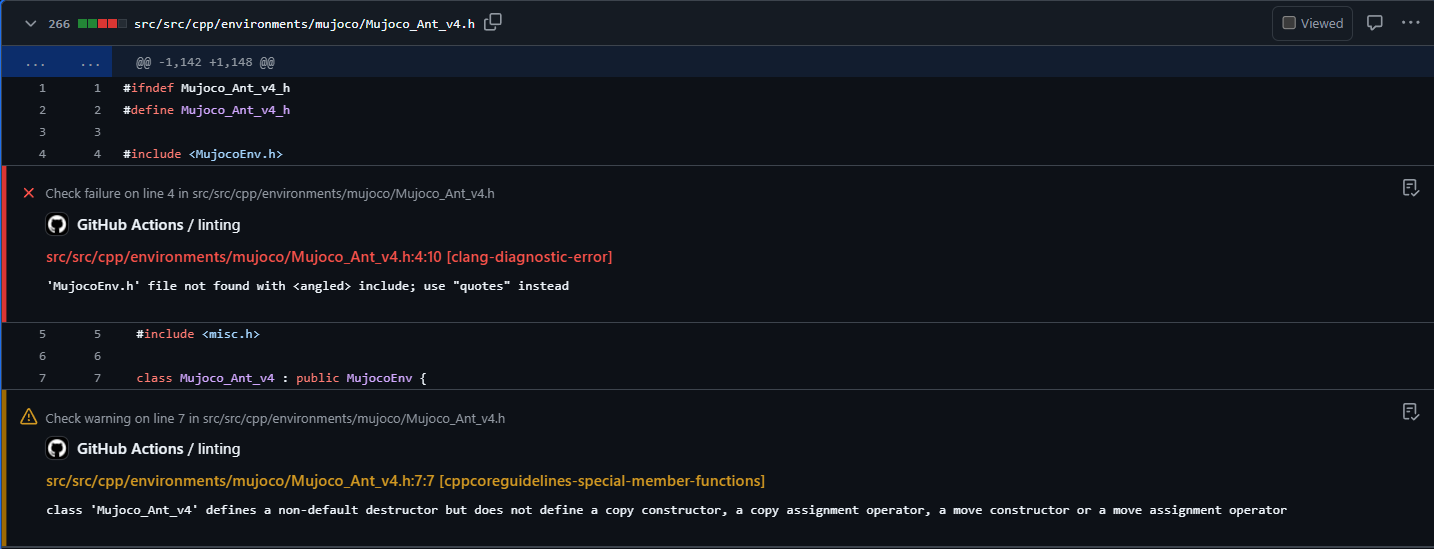
\includegraphics[width=1\textwidth]{linter-example.png}
  \caption{Example of a Linter Error}
  \label{fig:myimage}
\end{figure}

\section{Unit Testing}

\section{Changes Due to Testing}

% \wss{This section should highlight how feedback from the users and from 
% the supervisor (when one exists) shaped the final product.  In particular 
% the feedback from the Rev 0 demo to the supervisor (or to potential users) 
% should be highlighted.}
\subsection{Feedback from Rev 0}
The feedback given by the instructor and teaching assistant during Revision 0 was essential in guiding the next steps as the team looks toward the final demonstration.
Emphasis was placed on ensuring that usability testing was executed systematically rather than in the more ad-hoc manner initially planned by the team.
Some additional changes to be made include ensuring that unit testing and benchmarking of the implemented environments are cohesively executed and investigating whether the integration of deployment within the DRA is possible.

\section{Automated Testing}

As a result of the team’s conversion from building the project using SCons to CMake, automated testing became significantly easier to execute and debug.
To run any automated tests within a developer’s local environment, a developer can simply execute a command to build the project. 
This not only compiles everything but also runs all automated tests. If a developer wishes to run only the tests, they must navigate to the directory where the tests were already compiled (typically \texttt{/build/tests}). 
From there, the command \texttt{ctest} can be entered into the command prompt. Similar to the compilation process, all automated tests are executed once this command is run.\\

From the repository’s point of view, tests are executed using GitHub Actions or GitLab CI (depending on which repository is being viewed). 
Both linting and compilation are performed using the same commands that would be executed within a developer’s local environment. These tests run when a new pull request is made to the main branch, ensuring that all tests pass before merging.
The compiler workflow is also executed after merging into the main branch to ensure no errors or unintended changes in code behaviour have occurred. If any test or workflow fails, the logs of the workflow can be reviewed, providing a detailed summary of the reason for failure. 
This not only allows for easier debugging but also resolves the “works on my machine” issue.
		
\section{Trace to Requirements}
		
\section{Trace to Modules}		

\section{Code Coverage Metrics}

\bibliographystyle{plainnat}
\bibliography{../../refs/References}

\newpage{}
\section*{Appendix --- Reflection}

The information in this section will be used to evaluate the team members on the
graduate attribute of Reflection.

The purpose of reflection questions is to give you a chance to assess your own
learning and that of your group as a whole, and to find ways to improve in the
future. Reflection is an important part of the learning process.  Reflection is
also an essential component of a successful software development process.  

Reflections are most interesting and useful when they're honest, even if the
stories they tell are imperfect. You will be marked based on your depth of
thought and analysis, and not based on the content of the reflections
themselves. Thus, for full marks we encourage you to answer openly and honestly
and to avoid simply writing ``what you think the evaluator wants to hear.''

Please answer the following questions.  Some questions can be answered on the
team level, but where appropriate, each team member should write their own
response:


\begin{enumerate}
  \item What went well while writing this deliverable? 
  \item What pain points did you experience during this deliverable, and how
    did you resolve them?
  \item Which parts of this document stemmed from speaking to your client(s) or
  a proxy (e.g. your peers)? Which ones were not, and why?
  \item In what ways was the Verification and Validation (VnV) Plan different
  from the activities that were actually conducted for VnV?  If there were
  differences, what changes required the modification in the plan?  Why did
  these changes occur?  Would you be able to anticipate these changes in future
  projects?  If there weren't any differences, how was your team able to clearly
  predict a feasible amount of effort and the right tasks needed to build the
  evidence that demonstrates the required quality?  (It is expected that most
  teams will have had to deviate from their original VnV Plan.)
\end{enumerate}

\end{document}